\documentclass[a4paper,11pt]{article}
\usepackage{amsmath,amsthm,amsfonts,amssymb,amscd,amstext,vmargin,graphics,graphicx,tabularx,multicol} \usepackage[french]{babel}
\usepackage[utf8]{inputenc}  
\usepackage[T1]{fontenc} 
\usepackage[T1]{fontenc}
\usepackage{amsmath,amssymb}
\usepackage{pstricks-add,tikz,tkz-tab,variations}
\usepackage[autolanguage,np]{numprint} 
\usepackage{color}
\usepackage{ulem}

\setmarginsrb{1.5cm}{0.5cm}{1cm}{0.5cm}{0cm}{0cm}{0cm}{0cm} %Gauche, haut, droite, haut
\newcounter{numexo}
\newcommand{\exo}[1]{\stepcounter{numexo}\noindent{\bf Exercice~\thenumexo} : \marginpar{\hfill /#1}}
\reversemarginpar


\newcounter{enumtabi}
\newcounter{enumtaba}
\newcommand{\q}{\stepcounter{enumtabi} \theenumtabi)  }
\newcommand{\qa}{\stepcounter{enumtaba} (\alph{enumtaba}) }
\newcommand{\initq}{\setcounter{enumtabi}{0}}
\newcommand{\initqa}{\setcounter{enumtaba}{0}}

\newcommand{\be}{\begin{enumerate}}
\newcommand{\ee}{\end{enumerate}}
\newcommand{\bi}{\begin{itemize}}
\newcommand{\ei}{\end{itemize}}
\newcommand{\bp}{\begin{pspicture*}}
\newcommand{\ep}{\end{pspicture*}}
\newcommand{\bt}{\begin{tabular}}
\newcommand{\et}{\end{tabular}}
\renewcommand{\tabularxcolumn}[1]{>{\centering}m{#1}} %(colonne m{} centrée, au lieu de p par défault) 
\newcommand{\tnl}{\tabularnewline}

\newcommand{\trait}{\noindent \rule{\linewidth}{0.2mm}}
\newcommand{\hs}[1]{\hspace{#1}}
\newcommand{\vs}[1]{\vspace{#1}}

\newcommand{\N}{\mathbb{N}}
\newcommand{\Z}{\mathbb{Z}}
\newcommand{\R}{\mathbb{R}}
\newcommand{\C}{\mathbb{C}}
\newcommand{\Dcal}{\mathcal{D}}
\newcommand{\Ccal}{\mathcal{C}}
\newcommand{\mc}{\mathcal}

\newcommand{\vect}[1]{\overrightarrow{#1}}
\newcommand{\ds}{\displaystyle}
\newcommand{\eq}{\quad \Leftrightarrow \quad}
\newcommand{\vecti}{\vec{\imath}}
\newcommand{\vectj}{\vec{\jmath}}
\newcommand{\Oij}{(O;\vec{\imath}, \vec{\jmath})}
\newcommand{\OIJ}{(O;I,J)}

\newcommand{\bmul}[1]{\begin{multicols}{#1}}
\newcommand{\emul}{\end{multicols}}


\newcommand{\reponse}[1][1]{%
\multido{}{#1}{\makebox[\linewidth]{\rule[0pt]{0pt}{20pt}\dotfill}
}}

\newcommand{\titre}[5] 
% #1: titre #2: haut gauche #3: bas gauche #4: haut droite #5: bas droite
{
\noindent #2 \hfill #4 \\
#3 \hfill #5

\vspace{-1.6cm}

\begin{center}\rule{6cm}{0.5mm}\end{center}
\vspace{0.2cm}
\begin{center}{\large{\textbf{#1}}}\end{center}
\begin{center}\rule{6cm}{0.5mm}\end{center}
}



\begin{document}
\pagestyle{empty}
\titre{Contrôle 1 : Théorème de Pythagore, de Thalès et les fonctions }{Nom}{Prénom}{Date}{Classe}

\begin{flushleft}
\begin{tabular}{|m{9.5cm}|m{1.25cm}|m{1.25cm}|m{1.25cm}|m{1.25cm}|m{1.25cm}|}
\hline 
\textbf{Compétences} & \begin{center}
\textbf{N.E.}
\end{center} & \begin{center}
\textbf{M.I.}
\end{center} & \begin{center}
\textbf{M.F.}
\end{center}  & \begin{center}
\textbf{M.S.}
\end{center} & \begin{center}
\textbf{T.B.M.}
\end{center} \\ 
\hline 
Je dois savoir traduire en langage mathématique une situation réelle &  &  & & &\\
\hline 
Je dois savoir extraire d'un document les informations utiles, les reformuler, les organiser, les confronter à mes connaissances &  &  & & &\\
\hline
\end{tabular} 
\end{flushleft}

\textit{N.E = Non évalué ; M.I. = Maîtrise insuffisante ; M.F. = Maîtrise fragile ; M.S. = Maîtrise satisfaisante ; T.B.M. = Très bonne maîtrise}\\


\vspace*{0.25cm}
\textit{SUJET 2}\\

\exo{3} \\
Cet exercice est un questionnaire à choix multiples.\\
Pour chaque question, quatre réponses sont proposées mais une seule est exacte. Pour chacune des questions, entourer la bonne réponse, aucune justification n'est demandée.\\

\vspace*{0.25cm}

\renewcommand{\arraystretch}
{3.2}

\begin{tabular}{|c|p{9cm}|p{2.5cm}|p{2.35cm}|p{2.35cm}|}
\hline 
 & \textbf{Questions} & \textbf{Réponse B} & \textbf{Réponse B} & \textbf{Réponse C} \\ 
\hline 
\textbf{1} & La notation scientifique de 35 700 000 est : & $3,57 \times 10^{7}$ & $3,57 \times 10^{-7}$ & $35,7 \times 10^{6}$ \\
\hline 
\textbf{2} & $\dfrac{5}{3}-\dfrac{1}{3} \times \dfrac{3}{2}=$  : & $\dfrac{7}{6}$ & 2  & $\dfrac{2}{3}$ \\ 
\hline 
\textbf{3 }& $\dfrac{(10^{-3})^{2} \times 10^{5}}{10^{-7}}=$ & $10^{-8}$  & $10^{-7}$  & $10^{6}$   \\ 
\hline 
\end{tabular} 

\vspace*{1.5cm}

\exo{5} On considère la fonction suivante : $f(x)=-4x+7$\\
\renewcommand{\arraystretch}
{2}

\begin{tabular}{|p{1cm}|p{1cm}|p{1cm}|p{1cm}|p{1cm}|p{1cm}|p{1cm}|p{1cm}|p{1cm}|p{1cm}|}
\hline 
\textbf{x} & -3 & -2 & -1 & 0 & 1 & 2 & 3 & 4 & 5 \\ 
\hline 
\textbf{f(x)} & 19 & 15 & 11 & 7 & 3 & -1 & -5 & -9 & -13 \\ 
\hline 
\end{tabular} 

\vspace*{0.5cm}

Pour chacune des affirmations suivantes, indiquer si elle est vraie ou fausse. On rapelle que les réponses doivent être justifiées.\\

AFFIRMATION 1 : L'image de 3 par la fonction f est -5.\\

AFFIRMATION 2 : f(-1) = 2\\

AFFIRMATION 3 : L'antécédent de 35 par la fonction f est -8.\\

\newpage

\exo{3} Voisi la représentation graphique d'une fonction k.

\begin{center}
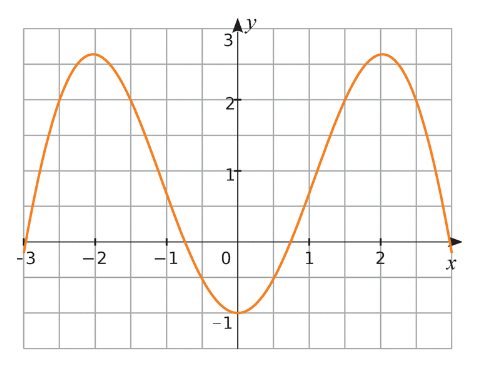
\includegraphics[scale=1.2]{fonction.eps} 
\end{center}

\noindent \initq \q Déterminer graphiquement les images de -0,5 et 1,5 par la fonction k.\\
\q Déterminer graphiquement le ou les antécédents de -0,5.\\
\q Est-il vrai que k(-2,5) = k(2,5) ? Jusitifier votre réponse.\\

\exo{3} Dans un coin de sa chambre mansardée, Lucie installe une étagère comme représentée sur le schéma ci-dessous. L'étagère est-elle parallèle au sol ?\\

\begin{center}

\includegraphics[scale=0.7]{recithales.eps} 
\end{center}

\vspace*{0.26cm}

\exo{6} 
Des élèves participent à une course à pied.\\
Avant l'épreuve, un plan leur a été remis.
Il est représenté par la figure ci-contre.\\
On convient que :\\
- Les droites (AE) et (BD) se coupent en C.\\
- Les droites (AB) et (DE) sont parallèles.\\
- ABC est un triangle rectangle en A.

\begin{center}
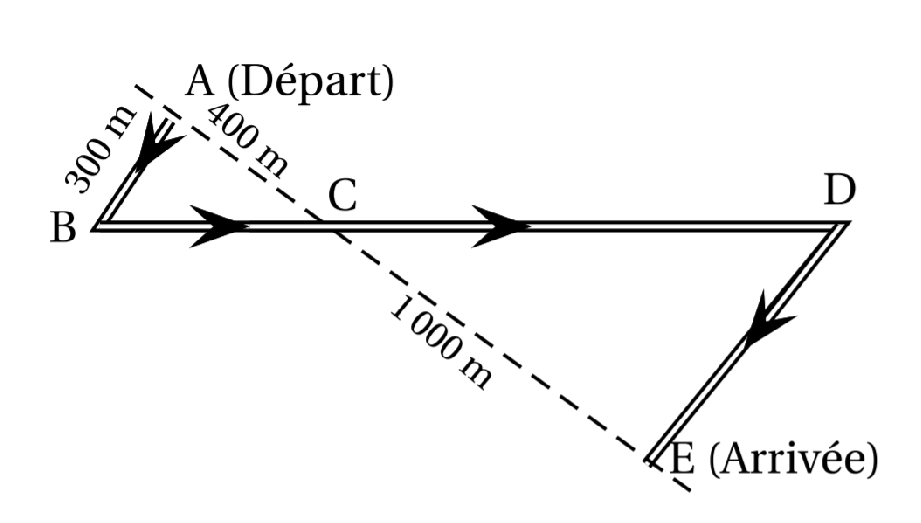
\includegraphics[scale=0.6]{thalesbrevet.eps} 
\end{center}

$\rightarrow$ \textbf{ Calculer la longueur réelle du parcours ABCDE.}\\
\textit{Si le travail n'est pas terminé, laisser tout de même une trace de la recherche. Elle sera
prise en compte dans la notation.}


\end{document}
